\documentclass[12pt,a4paper,oneside]{report} %<<<1 ------------------------------
% fonts, encoding:
\usepackage[utf8]{inputenc}             % file is in utf8:
\usepackage{cmap}                       % pdf is created with correct special characters, requires proper font, see next two lines
\usepackage[T1]{fontenc}                % see higher line
\usepackage{tgtermes}                   % high quality times font
\usepackage{textcomp}                   % proper micro sign for SI, use: \textmu, in equation: $\hbox{\textmu}$
\usepackage{slantsc}                   % proper micro sign for SI, use: \textmu, in equation: $\hbox{\textmu}$
\usepackage{calc}                   % provides \widthof
\usepackage{enumitem}                   % provides \begin{description} with settings []
\usepackage{color}                   % provides coloured text
% obrazky:
\usepackage{graphicx}                   % to insert pictures
\usepackage{grffile}                    % enables spaces in picture file names
\grffilesetup{ multidot=false, babel=false, encoding, inputencoding=utf8, filenameencoding=utf8, space=true}
\newcommand*{\FILEDOT}{.}                   % if picture file name containt dot (e.g. aaa.bbb.pdf), then TeX considers rest as filename extension, so dot must be written as follows: \includegraphics{aaa\FILEDOT bbb.eps}
% rest:
\usepackage[pdftex,
            unicode,
            pdfauthor={Q-Wave consorcium},
            pdftitle={Quantum Wave ToolBox documentation},
            pdfkeywords={algorithm, data procesing, sampling, toolbox},
            pdfproducer={Latex with hyperref},
            pdfcreator={pdflatex}]{hyperref}
%\usepackage[a4paper]{geometry}          % ensure A4
%\geometry{verbose,lmargin=2.5cm,rmargin=2.5cm,tmargin=2.5cm,bmargin=2.5cm}      % margins settings
\usepackage{url}                        % enables \url in bibtex
%\usepackage{setspace} \doublespacing   % double line spacing, for 1.5 set \onehalfspace
\usepackage{xspace}                     % proper automatic spacing after user defined commands
\usepackage{amsmath}                    % better equations

% lstlisting settings %<<<1 ----------------------------------------------------
\usepackage{listings}                   % for source code formatting
\definecolor{mygreen}{rgb}{0,0.6,0}
\definecolor{mygray}{rgb}{0.5,0.5,0.5}
\definecolor{lightgray}{rgb}{0.95,0.95,0.95}
\definecolor{mymauve}{rgb}{0.58,0,0.82}

\lstdefinestyle{mcode}{
%\lstset{ %
  backgroundcolor=\color{lightgray},   % choose the background color; you must add \usepackage{color} or \usepackage{xcolor}
  basicstyle=\normalsize\sffamily,        % the size of the fonts that are used for the code
  breakatwhitespace=false,         % sets if automatic breaks should only happen at whitespace
  breaklines=true,                 % sets automatic line breaking
  captionpos=b,                    % sets the caption-position to bottom
  commentstyle=\color{mygreen},    % comment style
  deletekeywords={...},            % if you want to delete keywords from the given language
  escapeinside={\%*}{*)},          % if you want to add LaTeX within your code
  extendedchars=true,              % lets you use non-ASCII characters; for 8-bits encodings only, does not work with UTF-8
  frame=single,	                   % adds a frame around the code
  keepspaces=true,                 % keeps spaces in text, useful for keeping indentation of code (possibly needs columns=flexible)
  keywordstyle=\color{blue},       % keyword style
  language=Matlab,                 % the language of the code
  otherkeywords={*,qwtb,alg_info,alg_wrapper,
        normrnd, alg_test,alg_example,...},           % if you want to add more keywords to the set
  numbers=none,                    % where to put the line-numbers; possible values are (none, left, right)
  numbersep=5pt,                   % how far the line-numbers are from the code
  numberstyle=\tiny\color{mygray}, % the style that is used for the line-numbers
  rulecolor=\color{black},         % if not set, the frame-color may be changed on line-breaks within not-black text (e.g. comments (green here))
  showspaces=false,                % show spaces everywhere adding particular underscores; it overrides 'showstringspaces'
  showstringspaces=false,          % underline spaces within strings only
  showtabs=false,                  % show tabs within strings adding particular underscores
  stepnumber=2,                    % the step between two line-numbers. If it's 1, each line will be numbered
  stringstyle=\color{mymauve},     % string literal style
  tabsize=2,                       % sets default tabsize to 2 spaces
  title=\lstname,                  % show the filename of files included with \lstinputlisting; also try caption instead of title
  belowskip=0pt                  % skip after end of lstlistings
}

\lstdefinestyle{output}{
%\lstset{ %
  backgroundcolor=\color{lightgray},   % choose the background color; you must add \usepackage{color} or \usepackage{xcolor}
  basicstyle=\normalsize\itshape,        % the size of the fonts that are used for the code
  breakatwhitespace=false,         % sets if automatic breaks should only happen at whitespace
  breaklines=true,                 % sets automatic line breaking
  captionpos=b,                    % sets the caption-position to bottom
  commentstyle=\color{mygreen},    % comment style
  deletekeywords={...},            % if you want to delete keywords from the given language
  escapeinside={\%*}{*)},          % if you want to add LaTeX within your code
  extendedchars=true,              % lets you use non-ASCII characters; for 8-bits encodings only, does not work with UTF-8
  frame=none,	                   % adds a frame around the code
  keepspaces=true,                 % keeps spaces in text, useful for keeping indentation of code (possibly needs columns=flexible)
  keywordstyle=\color{blue},       % keyword style
  language=Matlab,                 % the language of the code
  otherkeywords={*,qwtb,alg_info,alg_wrapper,alg_test,alg_example,...},           % if you want to add more keywords to the set
  numbers=none,                    % where to put the line-numbers; possible values are (none, left, right)
  numbersep=5pt,                   % how far the line-numbers are from the code
  numberstyle=\tiny\color{mygray}, % the style that is used for the line-numbers
  rulecolor=\color{black},         % if not set, the frame-color may be changed on line-breaks within not-black text (e.g. comments (green here))
  showspaces=false,                % show spaces everywhere adding particular underscores; it overrides 'showstringspaces'
  showstringspaces=false,          % underline spaces within strings only
  showtabs=false,                  % show tabs within strings adding particular underscores
  stepnumber=2,                    % the step between two line-numbers. If it's 1, each line will be numbered
  stringstyle=\color{mymauve},     % string literal style
  tabsize=2,                       % sets default tabsize to 2 spaces
  title=\lstname,                  % show the filename of files included with \lstinputlisting; also try caption instead of title
  belowskip=0pt,                  % skip after end of lstlistings
  xleftmargin=20pt                      % margin on left side
}

\lstset{style=mcode}
     % user defined code formatting

% bibliography settings %<<<1 ----------------------------------------------------
\usepackage[english]{babel} % main language of the document must be last
\usepackage[
   backend=biber      % if we want unicode 
  ,style=ieee   % or iso-numeric for numeric citation method          
  ,babel=other        % to support multiple languages in bibliography
  %,sortlocale=cs_CZ   % locale of main language, it is for sorting
  ,sortlocale=en_UK   % locale of main language, it is for sorting
  ,bibencoding=UTF8   % this is necessary only if bibliography file is in different encoding than main document
]{biblatex}

\bibliography{alllib2}
%\defbibenvironment{bibliography}
%    {\list
%        {[\printfield[labelnumberwidth]{labelnumber}]}
%        {\setlength{\labelwidth}{\labelnumberwidth}
%        \setlength{\leftmargin}{4pt}
%        \setlength{\labelsep}{10pt}
%        \addtolength{\leftmargin}{\labelsep}
%        \setlength{\itemsep}{6pt}
%        \setlength{\parsep}{\bibparsep}}
%        \renewcommand*{\makelabel}[1]{\hss##1}}
%    {\endlist}
%    {\item}

% shorts: %<<<1 ----------------------------------------------------

\def\Alg{{\sc Algorithm}\xspace}
\def\Algs{{\sc Algorithms}\xspace}
\def\Tb{{\sc Toolbox}\xspace}
\def\Da{{\sc Data}\xspace}
\def\Mea{{\sc Measurement}\xspace}
\def\Qua{{\sc Quantity}\xspace}
\def\Quas{{\sc Quantities}\xspace}
\def\Wr{{\sc Wrapper}\xspace}
\def\Wrs{{\sc Wrappers}\xspace}
\def\matlab{{\sc MATLAB}\xspace}
\def\octave{{\sc GNU Octave}\xspace}
\def\labview{{\sc LabVIEW}\xspace}
\def\mgo{\matlab/\octave\xspace}
        
\begin{document} % other document settings --------------------------------------------%<<<1
% how to devide special words, e.g. auto-mation
\hyphenation{Frame-work OpenOffice SourceForge Windows}
%\def\thesection{\Roman{section}}       % redefines numbering style of sections
\renewcommand\floatpagefraction{.9} \renewcommand\topfraction{.9} \renewcommand\bottomfraction{.9} \renewcommand\textfraction{.1} \setcounter{totalnumber}{50} \setcounter{topnumber}{50} \setcounter{bottomnumber}{50} % if too many pictures, change text/float fraction
\renewcommand{\labelitemi}{--}          % item sepparator
\setlength{\unitlength}{1mm}            % default length in picture environment

% tight description environment:
\newenvironment{tightdesc}{\begin{description}[itemsep=0pt]} 
                              {\end{description}}

% names of sections:
\def\infosection{Description}
\def\examplesection{Example}
% remove "chapter" from chapter heading:
\renewcommand{\chaptername}{}

\title{Quantum Wave ToolBox Algorithms documentation}
\author{Q-Wave consorcium}

% first page ----------------------------------------------------------------------- %<<<1 ------------------------------
\thispagestyle{empty}
\begin{center}
        \vspace*{10em}
        {\huge
        
\includegraphics[width=0.3\textwidth]{logo/qwtb_logo.png}

        \vspace{0.5em}
        Quantum Wave ToolBox\\

        \vspace{1.5em}
        Documentation of Algorithms}\\

        \vfill
        {\Large \color{red}{QWTB version 0.1}}

        \vspace{1em}
        {\Large \url{https://qwtb.github.io/qwtb/}}
\end{center}
\newpage

\tableofcontents

\chapter{Introduction} %<<<1 ------------------------------
This document gives overview of the algorithms implemented in Quantum Wave ToolBox (QWTB).

Toolbox was realized within the EMRP-Project SIB59 Q-Wave. The EMRP is jointly funded by the EMRP
par- ticipating countries within EURAMET and the European Union.

\vfill

\includegraphics[width=0.3\textwidth]{sources/Q-Wave_logo_01.pdf}
\hfill

\includegraphics[width=0.3\textwidth]{sources/eurametlogo.jpg}

\chapter{INL -- Integral Non-Linearity of ADC} %<<<1 ------------------------------
% included files are automatically generated by info_all_algs.m script and by Matlab publish
% function and converted by bash script betterpublish.
\section*{\infosection} %<<<2 -------------------
\begin{tightdesc}
\item [\textsf{.id}] --- INL
\item [\textsf{.name}] --- Integral Non-Linearity of ADC
\item [\textsf{.desc}] --- Calculates Integral Non-Linearity of an ADC. ADC has to sample sinewave, ADC codes are required.
\item [\textsf{.citation}] --- Virosztek, T., Pálfi V., Renczes B., Kollár I., Balogh L., Sárhegyi A., Márkus J., Bilau Z. T., ADCTest project site: \url{http://www.mit.bme.hu/projects/adctest} 2000-2014
\item [\textsf{.remarks}] --- Based on the ADCTest Toolbox v4.3, November 25, 2014.
\item [\textsf{.license}] --- UNKNOWN
\item [\textsf{.requires}] \rule{0em}{0em}
\begin{tightdesc}
\item [\textsf{t}] --- time series of sampled data
\item [\textsf{codes}] --- Sampled values represented as ADC codes (not converted to voltage)
\end{tightdesc}
\item [\textsf{.returns}] \rule{0em}{0em}
\begin{tightdesc}
\item [\textsf{INL}] --- INL
\end{tightdesc}
\item [\textsf{.providesGUF}] --- no
\item [\textsf{.providesMCM}] ---  no
\end{tightdesc}

\section*{\examplesection} %<<<2 ------------------------

% This LaTeX was auto-generated from an M-file by MATLAB.
% To make changes, update the M-file and republish this document.

%%% \documentclass{article}
%%% \usepackage{graphicx}
%%% \usepackage{color}

%%% \sloppy
%%% \definecolor{lightgray}{gray}{0.5}
\setlength{\parindent}{0pt}

%%% \begin{document}

    
    
\subsection*{Integral Non Linearity of ADC}

\begin{par}
Example for algorithm INL
\end{par} \vspace{1em}
\begin{par}
INL is an algorithm for estimating Integral Non-Linearity of an ADC. ADC has to sample sinewave, ADC codes are required.
\end{par} \vspace{1em}
\begin{par}
See also 'Virosztek, T., Pálfi V., Renczes B., Kollár I., Balogh L., Sárhegyi A., Márkus J., Bilau Z. T., ADCTest project site: \url{http://www.mit.bme.hu/projects/adctest} 2000-2014';
\end{par} \vspace{1em}

\subsubsection*{Contents}

\begin{itemize}
\setlength{\itemsep}{-1ex}
   \item Generate sample data
   \item Call algorithm
\end{itemize}


\subsubsection*{Generate sample data}

\begin{par}
Suppose a sine wave of nominal frequency 10 Hz and nominal amplitude 1 V is sampled by ADC with bit resolution of 4. First quantities \lstinline{t} with time of samples and quantity \lstinline{bits} with number of bits are prepared and put into input data structure \lstinline{DI}.
\end{par} \vspace{1em}
\begin{lstlisting}[style=mcode]
DI = [];
DI.t.v=[0:1/1e4:1-1/1e4];
DI.bits.v = 4;
\end{lstlisting}
\begin{par}
Waveform is constructed.
\end{par} \vspace{1em}
\begin{lstlisting}[style=mcode]
Anom = 1; fnom = 2; phnom = 0;
wvfrm = Anom*sin(2*pi*fnom*DI.t.v + phnom);
\end{lstlisting}
\begin{par}
Next code values are calculated. It is simulated by quantization and scaling of the sampled waveform. In real measurement code values can be obtained directly from the ADC. Suppose ADC range is -1..1.
\end{par} \vspace{1em}
\begin{lstlisting}[style=mcode]
codes = wvfrm;
rmin = -1; rmax = 1;
levels = 2.^DI.bits.v - 1;
codes(codes<rmin) = rmin;
codes(codes>rmax) = rmax;
codes = round((codes-rmin)./2.*levels);
\end{lstlisting}
\begin{par}
Now lets introduce ADC error. Instead of generating code 2 ADC erroneously generates code 3 and instead of 10 it generates 11.
\end{par} \vspace{1em}
\begin{lstlisting}[style=mcode]
codes(codes==2) = 3;
codes(codes==10) = 11;
codes = codes + min(codes);
\end{lstlisting}
\begin{par}
Create quantity \lstinline{codes} and plot a figure with sampled sine wave and codes.
\end{par} \vspace{1em}
\begin{lstlisting}[style=mcode]
DI.codes.v = codes;
figure
%plot(t, (y+1).*1/2.*levels, t, codes);
hold on
stairs(DI.t.v, codes);
wvfrm = (wvfrm + Anom).*levels./2;
plot(DI.t.v, wvfrm, '-r');
xlabel('t (s)')
ylabel('Codes / Voltage (scaled)');
legend('Codes generated by ADC','Original waveform scaled to match codes');
hold off
\end{lstlisting}

\begin{center}
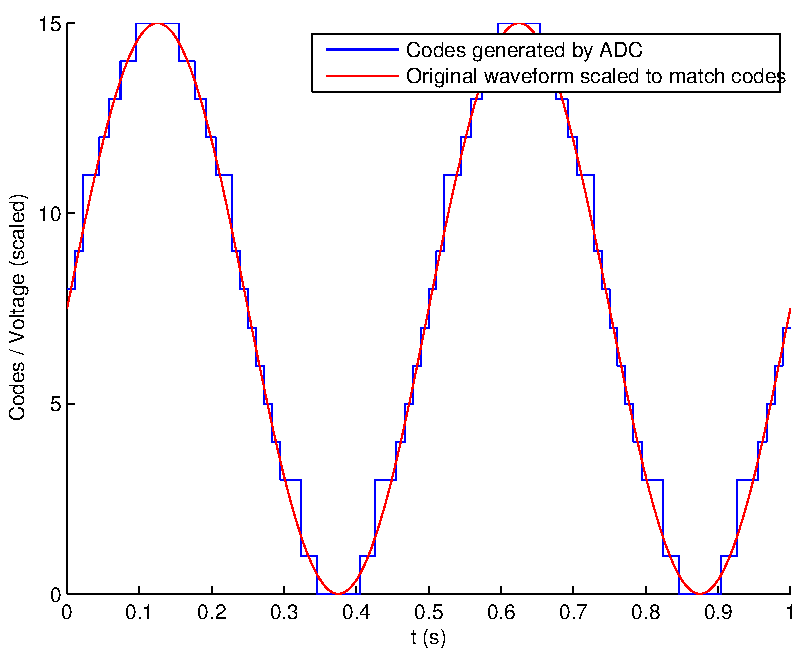
\includegraphics[width=0.7\textwidth]{alg_examples_published/INL_alg_example_01.pdf}
\end{center}


\subsubsection*{Call algorithm}

\begin{par}
Apply INL algorithm to the input data \lstinline{DI}.
\end{par} \vspace{1em}
\begin{lstlisting}[style=mcode]
DO = qwtb('INL', DI);
\end{lstlisting}

        \begin{lstlisting}[style=output]
QWTB: no uncertainty calculation
\end{lstlisting} \color{black}
    \begin{par}
Plot results of integral non-linearity. One can clearly observe defects on codes 3 and 11.
\end{par} \vspace{1em}
\begin{lstlisting}[style=mcode]
figure
plot(DO.INL.v, '-x');
xlabel('Code value')
ylabel('INL')
\end{lstlisting}

\begin{center}
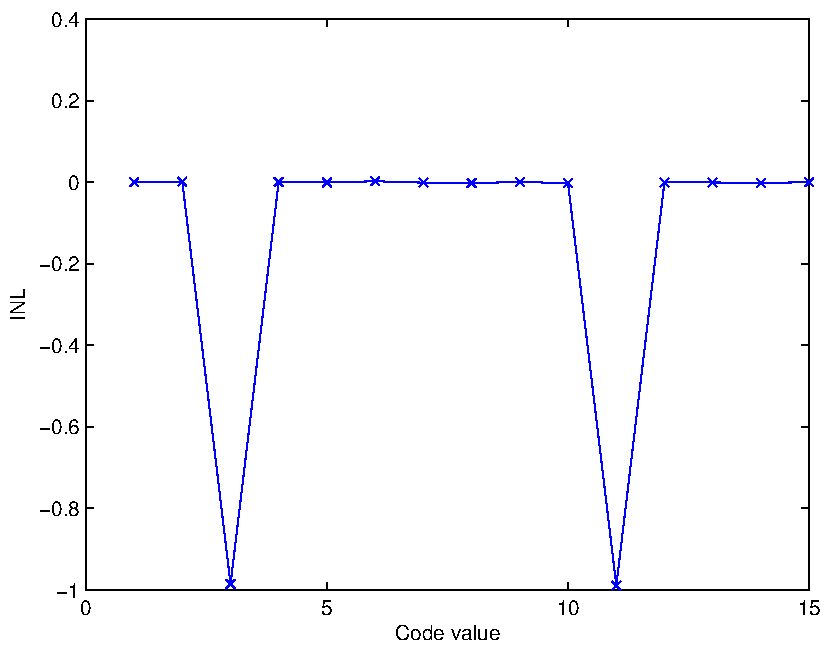
\includegraphics[width=0.7\textwidth]{alg_examples_published/INL_alg_example_02.pdf}
\end{center}



%%% \end{document}
    


\chapter{PSFE -- Phase Sensitive Frequency Estimator} %<<<1 ------------------------------
% included files are automatically generated by info_all_algs.m script and by Matlab publish
% function and converted by bash script betterpublish.
\section*{\infosection} %<<<2 -------------------
\begin{tightdesc}
\item [Id:] PSFE
\item [Name:] Phase Sensitive Frequency Estimator
\item [Description:] An algorithm for estimating the frequency, amplitude, and phase of the fundamental component in harmonically distorted waveforms. The algorithm minimizes the phase difference between the sine model and the sampled waveform by effectively minimizing the influence of the harmonic components. It uses a three-parameter sine-fitting algorithm for all phase calculations. The resulting estimates show up to two orders of magnitude smaller sensitivity to harmonic distortions than the results of the four-parameter sine fitting algorithm.
\item [Citation:] Lapuh, R., "Estimating the Fundamental Component of Harmonically Distorted Signals From Noncoherently Sampled Data," Instrumentation and Measurement, IEEE Transactions on , vol.64, no.6, pp.1419,1424, June 2015, doi: 10.1109/TIM.2015.2401211, URL: \url{http://ieeexplore.ieee.org/stamp/stamp.jsp?tp=\&arnumber=7061456\&isnumber=7104190}
\item [Remarks:] If sampling time |Ts| is not supplied, wrapper will calculate |Ts| from sampling frequency |fs| or if not supplied, mean of differences of time series |t| is used to calculate |Ts|.
\item [License:] MIT License
\item [Provides GUF:] no
\item [Provides MCM:] no
\item [Input Quantities] \rule{0em}{0em}
    \begin{tightdesc}
    \item [Required:] 
        \textsf{Ts} or \textsf{fs} or \textsf{t},\enspace \textsf{y}
    \item [Descriptions:] \rule{0em}{0em}
        \begin{tightdesc}
            \item[\textsf{Ts}] -- Sampling time
            \item[\textsf{fs}] -- Sampling frequency
            \item[\textsf{t}] -- Time series
            \item[\textsf{y}] -- Sampled values
        \end{tightdesc}
    \end{tightdesc}
\item [Output Quantities:] \rule{0em}{0em}
    \begin{tightdesc}
        \item[\textsf{A}] -- Amplitude of main signal component
        \item[\textsf{f}] -- Frequency of main signal component
        \item[\textsf{ph}] -- Phase of main signal component
    \end{tightdesc}
\end{tightdesc}

\section*{\examplesection} %<<<2 ------------------------

% This LaTeX was auto-generated from an M-file by MATLAB.
% To make changes, update the M-file and republish this document.

%%% \documentclass{article}
%%% \usepackage{graphicx}
%%% \usepackage{color}

%%% \sloppy
%%% \definecolor{lightgray}{gray}{0.5}
\setlength{\parindent}{0pt}

%%% \begin{document}

    
    
\subsection*{Phase Sensitive Frequency Estimator}

\begin{par}
Example for algorithm PSFE.
\end{par} \vspace{1em}
\begin{par}
PSFE is an algorithm for estimating the frequency, amplitude, and phase of the fundamental component in harmonically distorted waveforms. The algorithm minimizes the phase difference between the sine model and the sampled waveform by effectively minimizing the influence of the harmonic components. It uses a three-parameter sine-fitting algorithm for all phase calculations. The resulting estimates show up to two orders of magnitude smaller sensitivity to harmonic distortions than the results of the four-parameter sine fitting algorithm.
\end{par} \vspace{1em}
\begin{par}
See also Lapuh, R., "Estimating the Fundamental Component of Harmonically Distorted Signals From Noncoherently Sampled Data," Instrumentation and Measurement, IEEE Transactions on , vol.64, no.6, pp.1419,1424, June 2015, doi: 10.1109/TIM.2015.2401211, URL: \url{http://ieeexplore.ieee.org/stamp/stamp.jsp?tp=&arnumber=7061456&isnumber=7104190}'
\end{par} \vspace{1em}

\subsubsection*{Contents}

\begin{itemize}
\setlength{\itemsep}{-1ex}
   \item Generate sample data
   \item Call algorithm
   \item Display results
\end{itemize}


\subsubsection*{Generate sample data}

\begin{par}
Two quantities are prepared: \lstinline{t} and \lstinline{y}, representing 1 second of sinus waveform of nominal frequency 100 Hz, nominal amplitude 1 V and nominal phase 1 rad, sampled at sampling frequency 10 kHz.
\end{par} \vspace{1em}
\begin{lstlisting}[style=mcode]
DI = [];
Anom = 1; fnom = 100; phnom = 1;
DI.t.v = [0:1/1e4:1-1/1e4];
DI.y.v = Anom*sin(2*pi*fnom*DI.t.v + phnom);
\end{lstlisting}
\begin{par}
Add noise:
\end{par} \vspace{1em}
\begin{lstlisting}[style=mcode]
DI.y.v = DI.y.v + normrnd(0, 1e-3, size(DI.y.v));
\end{lstlisting}


\subsubsection*{Call algorithm}

\begin{par}
Use QWTB to apply algorithm \lstinline{PSFE} to data \lstinline{DI}.
\end{par} \vspace{1em}
\begin{lstlisting}[style=mcode]
DO = qwtb('PSFE', DI);
\end{lstlisting}

        \begin{lstlisting}[style=output]
QWTB: no uncertainty calculation
\end{lstlisting} \color{black}
    

\subsubsection*{Display results}

\begin{par}
Results is the amplitude, frequency and phase of sampled waveform.
\end{par} \vspace{1em}
\begin{lstlisting}[style=mcode]
f = DO.f.v
A = DO.A.v
ph = DO.ph.v
\end{lstlisting}

        \begin{lstlisting}[style=output]

f =

  100.0000


A =

    1.0000


ph =

    1.0000

\end{lstlisting} \color{black}
    \begin{par}
Errors of estimation in parts per milion:
\end{par} \vspace{1em}
\begin{lstlisting}[style=mcode]
ferrppm = (DO.f.v - fnom)/fnom .* 1e6
Aerrppm = (DO.A.v - Anom)/Anom .* 1e6
pherrppm = (DO.ph.v - phnom)/phnom .* 1e6
\end{lstlisting}

        \begin{lstlisting}[style=output]

ferrppm =

    0.1113


Aerrppm =

    4.3774


pherrppm =

  -13.7952

\end{lstlisting} \color{black}
    


%%% \end{document}
    


\chapter{FPSWF -- Four Parameter Sine Wave Fitting} %<<<1 ------------------------------
% included files are automatically generated by info_all_algs.m script and by Matlab publish
% function and converted by bash script betterpublish.
\section*{\infosection} %<<<2 -------------------
\begin{tightdesc}
\item [\textsf{.id}] --- FPSWF
\item [\textsf{.name}] --- Four Parameter Sine Wave Fit
\item [\textsf{.desc}] --- Fits a sine wave to the recorded data by means of least squares fitting using 4 parameter (frequency, amplitude, phase and offset) model. An estimate of signal frequency is required. Due to non-linear characteristic, converge is not always achieved. When run in Matlab, function `lsqnonlin` in Optimization toolbox is used. When run in GNU Octave, function `leasqr` in GNU Octave Forge package optim is used.
\item [\textsf{.citation}] --- 
\item [\textsf{.remarks}] --- Algorithm works essentially only for simple sine wave. Algorithm is very sensitive to distortion. Algorithm requires good estimate of signal frequency.
\item [\textsf{.license}] --- MIT License
\item [\textsf{.requires}] \rule{0em}{0em}
\begin{tightdesc}
\item [\textsf{t}] --- Time series of sampled data
\item [\textsf{y}] --- Sampled values
\item [\textsf{fest}] --- Estimate of signal frequency
\end{tightdesc}
\item [\textsf{.returns}] \rule{0em}{0em}
\begin{tightdesc}
\item [\textsf{f}] --- Frequency of main signal component
\item [\textsf{A}] --- Amplitude of main signal component
\item [\textsf{ph}] --- Phase of main signal component
\item [\textsf{O}] --- Offset of signal
\end{tightdesc}
\item [\textsf{.providesGUF}] --- no
\item [\textsf{.providesMCM}] ---  no
\end{tightdesc}

\section*{\examplesection} %<<<2 ------------------------

% This LaTeX was auto-generated from an M-file by MATLAB.
% To make changes, update the M-file and republish this document.

%%% \documentclass{article}
%%% \usepackage{graphicx}
%%% \usepackage{color}

%%% \sloppy
%%% \definecolor{lightgray}{gray}{0.5}
\setlength{\parindent}{0pt}

%%% \begin{document}

    
    
\subsection*{Four parameter sine wave fitting}

\begin{par}
Example for algorithm FPSWF.
\end{par} \vspace{1em}
\begin{par}
FPSWF is an algorithm for estimating the frequency, amplitude, and phase of the sine waveform. The algorithm use least squares method. Algorithm requires good estimate of frequency.
\end{par} \vspace{1em}

\subsubsection*{Contents}

\begin{itemize}
\setlength{\itemsep}{-1ex}
   \item Generate sample data
   \item Call algorithm
   \item Display results
\end{itemize}


\subsubsection*{Generate sample data}

\begin{par}
Two quantities are prepared: \lstinline{t} and \lstinline{y}, representing 1 second of sinus waveform of nominal frequency 1 kHz, nominal amplitude 1 V, nominal phase 1 rad and offset 1 V sampled at sampling frequency 10 kHz.
\end{par} \vspace{1em}
\begin{lstlisting}[style=mcode]
DI = [];
Anom = 2; fnom = 100; phnom = 1; Onom = 0.2;
DI.t.v = [0:1/1e4:1-1/1e4];
DI.y.v = Anom*sin(2*pi*fnom*DI.t.v + phnom) + Onom;
\end{lstlisting}
\begin{par}
Lets make an estimate of frequency 0.2 percent higher than nominal value:
\end{par} \vspace{1em}
\begin{lstlisting}[style=mcode]
DI.f.v = 100.2;
\end{lstlisting}


\subsubsection*{Call algorithm}

\begin{par}
Use QWTB to apply algorithm \lstinline{FPSWF} to data \lstinline{DI}.
\end{par} \vspace{1em}
\begin{lstlisting}[style=mcode]
CS.verbose = 1;
DO = qwtb('FPSWF', DI, CS);
\end{lstlisting}

        \begin{lstlisting}[style=output]
QWTB: no uncertainty calculation
Fitting started

Local minimum found.

Optimization completed because the size of the gradient is less than
the default value of the function tolerance.



Fitting finished
\end{lstlisting} \color{black}
    

\subsubsection*{Display results}

\begin{par}
Results is the amplitude, frequency and phase of sampled waveform.
\end{par} \vspace{1em}
\begin{lstlisting}[style=mcode]
A = DO.A.v
f = DO.f.v
ph = DO.ph.v
O = DO.O.v
\end{lstlisting}

        \begin{lstlisting}[style=output]

A =

    2.0000


f =

  100.0000


ph =

    1.0000


O =

   -0.2000

\end{lstlisting} \color{black}
    \begin{par}
Errors of estimation in parts per milion:
\end{par} \vspace{1em}
\begin{lstlisting}[style=mcode]
Aerrppm = (DO.A.v - Anom)/Anom .* 1e6
ferrppm = (DO.f.v - fnom)/fnom .* 1e6
pherrppm = (DO.ph.v - phnom)/phnom .* 1e6
Oerrppm = (DO.O.v - Onom)/Onom .* 1e6
\end{lstlisting}

        \begin{lstlisting}[style=output]

Aerrppm =

   4.8894e-07


ferrppm =

  -1.4211e-10


pherrppm =

   1.7542e-08


Oerrppm =

  -2.0000e+06

\end{lstlisting} \color{black}
    


%%% \end{document}
    


\chapter{SP-FFT -- Spectrum by means of Fast Fourier Transform} %<<<1 ------------------------------
% included files are automatically generated by info_all_algs.m script and by Matlab publish
% function and converted by bash script betterpublish.
\section*{\infosection} %<<<2 -------------------
\begin{tightdesc}
\item [\textsf{.id}] --- SP-FFT
\item [\textsf{.name}] --- Spectrum by means of Fast Fourier Transform
\item [\textsf{.desc}] --- Calculates frequency and phase spectrum by means of Fast Fourier Transform algorithm. Result is normalized.
\item [\textsf{.citation}] --- 
\item [\textsf{.remarks}] --- 
\item [\textsf{.license}] --- MIT License
\item [\textsf{.requires}] \rule{0em}{0em}
\begin{tightdesc}
\item [\textsf{y}] --- Sampled values
\item [\textsf{fs}] --- Sampling frequency
\end{tightdesc}
\item [\textsf{.returns}] \rule{0em}{0em}
\begin{tightdesc}
\item [\textsf{f}] --- Frequency series
\item [\textsf{A}] --- Amplitude series
\item [\textsf{ph}] --- Phase series
\end{tightdesc}
\item [\textsf{.providesGUF}] --- no
\item [\textsf{.providesMCM}] ---  no
\end{tightdesc}

\section*{\examplesection} %<<<2 ------------------------

% This LaTeX was auto-generated from an M-file by MATLAB.
% To make changes, update the M-file and republish this document.

%%% \documentclass{article}
%%% \usepackage{graphicx}
%%% \usepackage{color}

%%% \sloppy
%%% \definecolor{lightgray}{gray}{0.5}
\setlength{\parindent}{0pt}

%%% \begin{document}

    
    
\subsection*{Signal Spectrum by means of Fast fourier transform}

\begin{par}
Example for algorithm SP-FFT.
\end{par} \vspace{1em}
\begin{par}
Calculates frequency and phase spectrum by means of Fast Fourier Transform algorithm. Result is normalized.
\end{par} \vspace{1em}

\subsubsection*{Contents}

\begin{itemize}
\setlength{\itemsep}{-1ex}
   \item Generate sample data
   \item Call algorithm
   \item Display results
\end{itemize}


\subsubsection*{Generate sample data}

\begin{par}
Two quantities are prepared: \lstinline{y} and \lstinline{fs}, representing 1 second of signal containing 5 harmonic components and one inter-harmonic component. Main signal component has nominal frequency 1 kHz, nominal amplitude 2 V, nominal phase 1 rad and offset 1 V sampled at sampling frequency 10 kHz.
\end{par} \vspace{1em}
\begin{lstlisting}[style=mcode]
DI = [];
fsnom = 1e4; Anom = 2; fnom = 100; phnom = 1; Onom = 0.2;
t = [0:1/fsnom:1-1/fsnom];
DI.y.v = Anom*sin(2*pi*fnom*t + phnom);
for i = 2:45
        DI.y.v = DI.y.v + Anom./i*sin(2*pi*fnom*i*t + phnom + i - 1);
end
DI.y.v = DI.y.v + 1*sin(2*pi*fnom*1.456*t + phnom);
DI.fs.v = fsnom;
\end{lstlisting}


\subsubsection*{Call algorithm}

\begin{par}
Use QWTB to apply algorithm \lstinline{SP-FFT} to data \lstinline{DI}.
\end{par} \vspace{1em}
\begin{lstlisting}[style=mcode]
DO = qwtb('SP-FFT', DI);
\end{lstlisting}

        \begin{lstlisting}[style=output]
QWTB: no uncertainty calculation
\end{lstlisting} \color{black}
    

\subsubsection*{Display results}

\begin{par}
Results is the amplitude and phase spectrum.
\end{par} \vspace{1em}
\begin{lstlisting}[style=mcode]
figure
plot(DO.f.v, DO.A.v, '-x')
xlabel('f (Hz)'); ylabel('A (V)'); title('Amplitude spectrum of the signal');
figure
plot(DO.f.v, DO.ph.v, '-x')
xlabel('f (Hz)'); ylabel('phase (rad)'); title('Phase spectrum of the signal');
\end{lstlisting}

\begin{center}
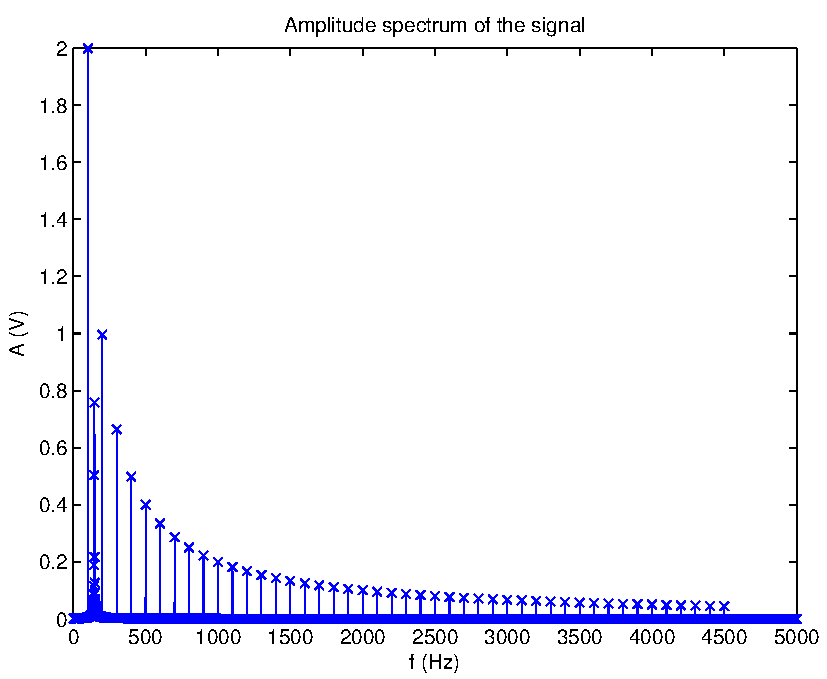
\includegraphics[width=0.7\textwidth]{algs_examples_published/SP-FFT_alg_example_01.pdf}
\end{center}

\begin{center}
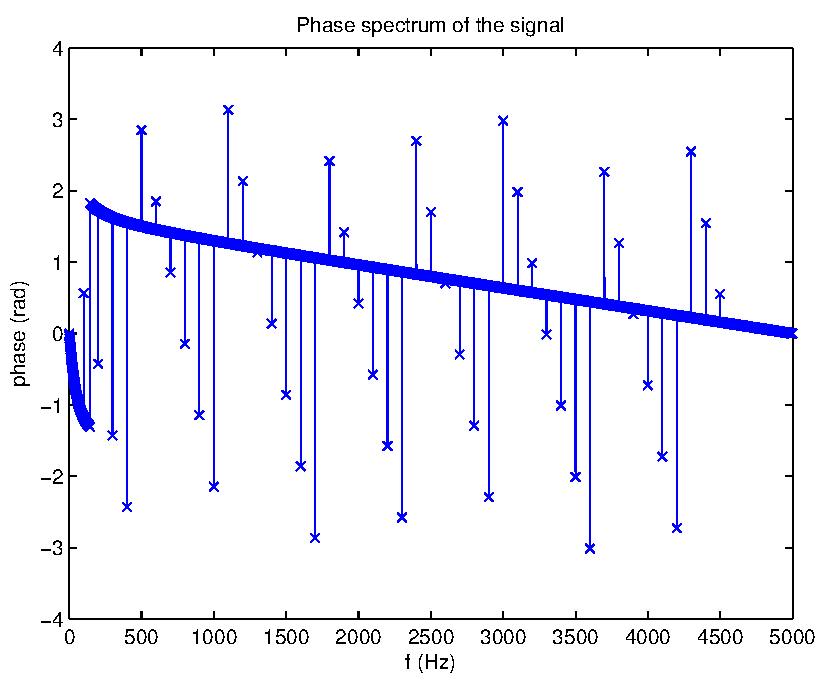
\includegraphics[width=0.7\textwidth]{algs_examples_published/SP-FFT_alg_example_02.pdf}
\end{center}



%%% \end{document}
    


\end{document}

% vim settings: vim:foldmarker=%<<<,%>>> fdm=marker fen
